\documentclass[]{article}
\usepackage{caption}
\usepackage{subcaption}
\usepackage{graphicx}
\usepackage{float}
\usepackage{url}
\usepackage{amsmath}
\usepackage{amssymb}
\usepackage{tocloft}
\usepackage{wasysym}
\usepackage[shortlabels]{enumitem}
\usepackage[hidelinks]{hyperref}
\usepackage[toc,acronym,nonumberlist]{glossaries}
\setacronymstyle{long-short}
\usepackage{glossaries-extra}
\usepackage[table]{xcolor}

\graphicspath{{figs/}} 
\setlength{\cftsubsecindent}{0em}
\setlength{\cftsecnumwidth}{3em}
\setlength{\cftsubsecnumwidth}{3em}
\newcommand\numberthis{\addtocounter{equation}{1}\tag{\theequation}}

%opening
\title{
	Origins of Life Course\\
	Peer Review Assignment
}

\makeglossaries
\loadglsentries{glossary-entries}

\begin{document}

\maketitle

\tableofcontents
\listoffigures

\section{Early systems chemistry}

Figure \ref{fig:damer} shows an early protocell cycle. Identify the following parts that are
required for a biological life cycle within the figure:
\begin{table}[H]
	\caption{Early systems chemistry}	{\rowcolors{1}{green!80!yellow!50}{green!70!yellow!40}
	\begin{tabular}{|c|p{3cm}|p{8cm}|}\hline
	a&	What is the individual? &The stabilized protocell is an individual.\\
	b&	Where in the cycle are metabolic processes occurring? &\\
	c&	How does selection occur? &Just after the head of the arrow labelled labelled "influx of solutes", during the Gel phase.\\
	d&	Is there reproduction? Why or why not? &Yes. Protocells are instantead at end of anhydrous phase.\\
	e&	What is one energetic input found in this system?&Evaporation, which drives dehydration\cite{damer2016field}\\\hline
	\end{tabular}}
\end{table}

\begin{figure}[H]
	\caption[Early protocell cycle]{Early protocell cycle after \cite{damer2016field}}\label{fig:damer}
	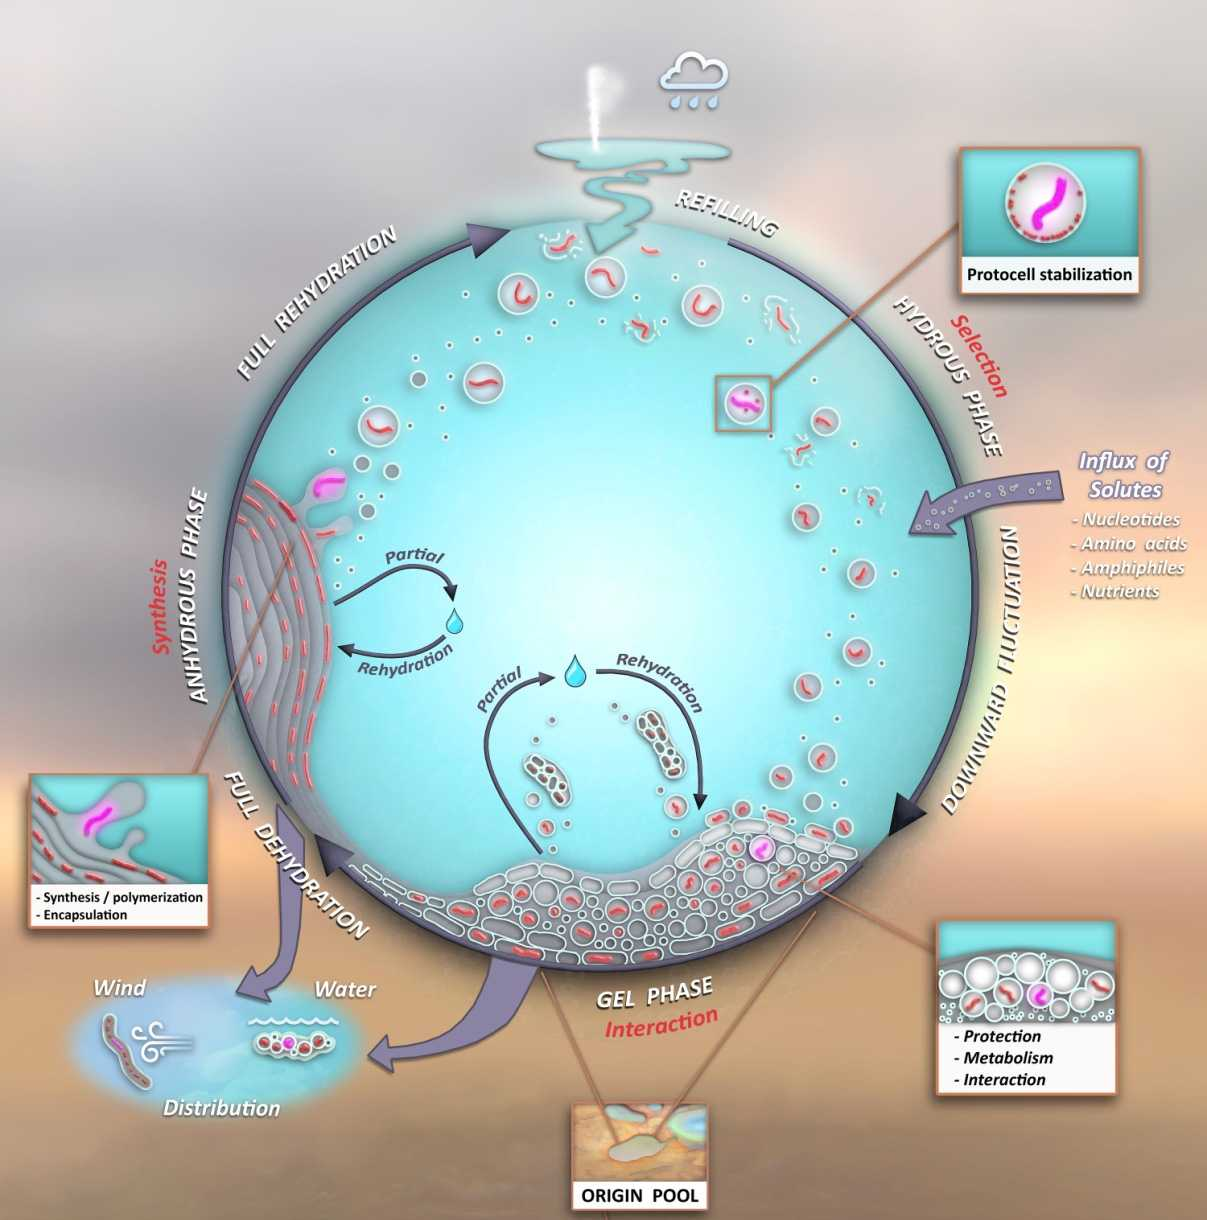
\includegraphics[width=\textwidth]{WarmLittlePond}
\end{figure}
\section{Time machine}

\begin{table}[H]
	\caption{My recommendations for Time Machine}
	{\rowcolors{1}{green!80!yellow!50}{green!70!yellow!40}
	\begin{tabular}{|c|p{3cm}|p{8cm}| } \hline
		a&What time... would you recommend they visit? &I'd be very interested in a time between 3.8 Gya and 3.5 Gya, as an intriguing but controversial case has been made for the existence of life \cite{mojzsis1996evidence,nutman2016rapid} in the Isua Greenstone belt \cite{enwiki:1095301862}--Figure \ref{fig:nuuk}. Mojzsis\cite{mojzsis1996evidence} pointed out that microfossils from 3.5 Gya were already complex, implying that there had already been considerable evolution, so a date close to 3.8 Gya would be good.\\
		b& What type of information would you want from the early Earth conditions at that
		time?& I'd like to know the atmospheric composition (especially $CO_2$, $NH_3$, and $CH_4$ ), and the the temperatures sampled during the time of the visit (which, I tryust, would not be less than one day).\\
		c& Is there a specific location/latitude you would recommend, or environment to sample		from? &(1 point)\\
		d& What criteria would you use to tell if the sample was “alive” or once was alive? &(1	point)\\\hline
	\end{tabular}}
\end{table}
\begin{figure}[H]
	\caption{Nuuk region after \cite{enwiki:1095301862}}\label{fig:nuuk}
	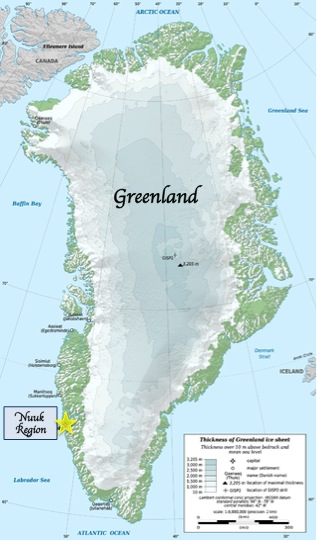
\includegraphics[width=\textwidth]{Nuuk_Location}
\end{figure}
\section{Phylogenetic tree building}
Phylogenetic tree building \cite{altschul1990basic}
\begin{enumerate}[(a)]
	\item Generate a phylogenetic tree based on a single protein (or nucleotide) sequence (1
point)
	\item Generate a phylogenetic tree based on the known taxonomy (1 point)
	\item Compare your protein and taxonomic trees. Do you notice any differences?
(Include at least 1 difference, or state that they are identical). (1 point)
	\item What are the challenges with building these trees? (Provide a minimum of 2
challenges) (2 points
\end{enumerate}


% glossary
\printglossaries

% bibliography go here

\bibliographystyle{unsrt}
\addcontentsline{toc}{section}{Bibliography}
\bibliography{origins,wikipedia}

\end{document}
